Straw tubes are proportional gaseous drift detectors. They consist of a gas filled conducting tube and a wire stretched along the tube axis. When charged particles pass through the straw tube, they interact electromagnetically with the gas atoms and molecules. These Coulomb interactions result in the creation of electron-ion pairs. Applying an electric field between the wire and the tube causes the electrons and ions to drift through the gas. The wire is usually biased to a positive voltage of a few kV and collects the electrons while the ions drift toward the tube wall as the cathode. The electric field strength near the anode wire is strong enough so that primary electrons obtain enough energy between collisions to produce secondary ionization electron-ion pairs in the gas. The produced electrons continue to drift and ionize more gas molecules and hence form an avalanche. When this avalanche reaches the anode wire it is large enough to produce a measurable signal to be recorded by the readout electronics. Because the straw tubes operate in the proportional region, the size of the signal is proportional to the originally deposited charge.
\section{Gas System for STS}
The straw tubes of detector are filled with CO$_{2}$ and Ar (80:20 or 90:10)  with different proportion and pressure . Thus to keep the pressure and proportion of gasses under constant over time. A very reliable and secure gas system is needed. The gas system was build in IFJ -PAN bronowice center and Jaggiellonia Univerty krakow. My task was to develop interface between computer and flow meter, pressure gauges to change different values of flow values and pressure. Also to developed  automated system using EPICS (Experimental Physics and Industrial Control System). I also created graphical user interface using Control System Studio (CS-Studio) see figure \ref{fig:fig5.1}.  
\begin{figure}
    \centering
    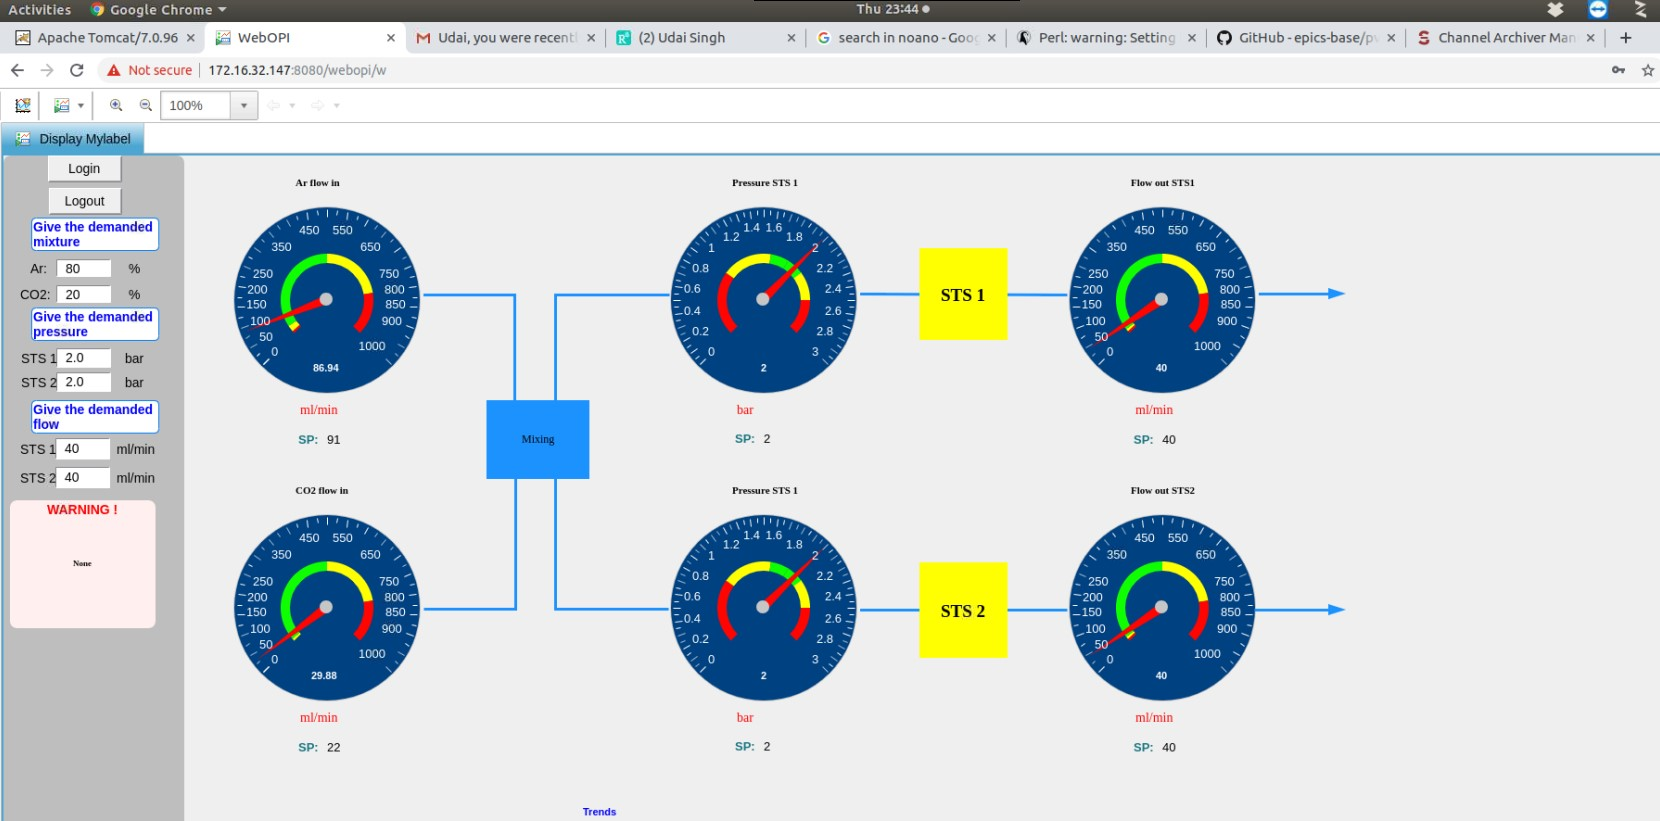
\includegraphics[width=1.0\textwidth]{images/webopi.jpg}
    \caption{Showing graphical user interface for the gas system}
    \label{fig:fig5.1}
\end{figure}
\subsection{Gas System software using EPICS}
\subsubsection{Hardware Platform}
For the gas system hardware two Bronhorst pressure gauge and four flow meter , and rarpberry pi3 bord is choosen to take control of six Bronhorst devices through R232 cable.
List of devices used in Gas System
\begin{itemize}
    \item Two bronkhorst pressure control : to control the pressure in both the straw tube detectors.
    \item Four flow meters: Two flow meter are needed for controling the flow of CO$_{2}$  and Ar flow in required propotions. And othre two are needed for the controling the ouput flow of the detectors.
    \item R232 cables: to inter connect the flow meter and pressure guage and power supply unit.
    \item R232 to USB adapter: to connect the raspberry pi to flow meters.
    \item A raspberry pi3 Board: To run EPICS program and cotrolling pressure gauge and flow meters.
    \item A computer: to use as gui interface out side the lab.
    \end{itemize}

\subsubsection{Software}
In the software development for the gas system we need two component's. One is controller to control all input output between raspberry pi and Gas System components. Second is Graphic user interface for the user.
In our case EPICS is used to develop such kind of controller. The following algorithm is used in this program.
\begin{itemize}
    \item Using Async driver and stream device is used to create I/O comunication between gas system componet and EPICS.
    \item In EPICS a .proto file is created in different command is written to set flow value (pressure in case pf pressure controler) or get the value from flow meter.
\end{itemize}



EPICS is used to control the flow meter and pressure guage. The CS-Studio is used as client to provide the graphical user interface(GUI) to users.
\begin{figure}
    \centering
    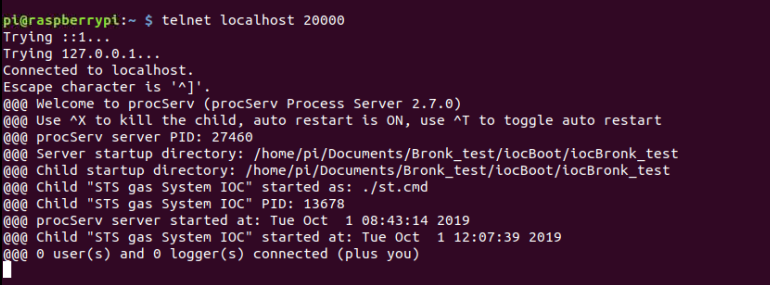
\includegraphics[width=1\textwidth]{images/procserv.PNG}
    \caption{Caption}
    \label{fig:my_label}
\end{figure}
\begin{figure}
    \centering
    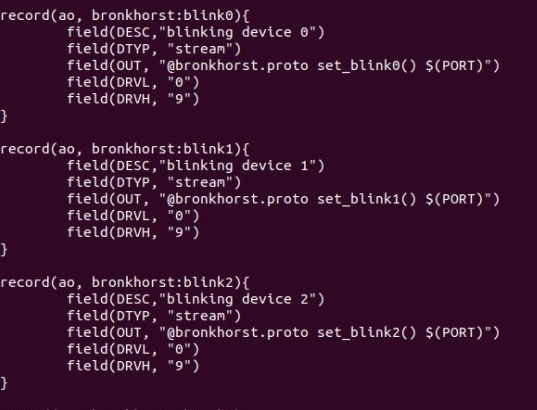
\includegraphics[width=1\textwidth]{images/dbrecord.jpg}
    \caption{Caption}
    \label{fig:my_label}
\end{figure}
\begin{figure}
    \centering
    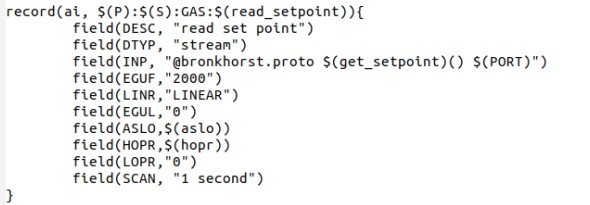
\includegraphics[width=1\textwidth]{images/subsitution.jpg}
    \caption{Caption}
    \label{fig:my_label}
\end{figure}
\begin{figure}
    \centering
    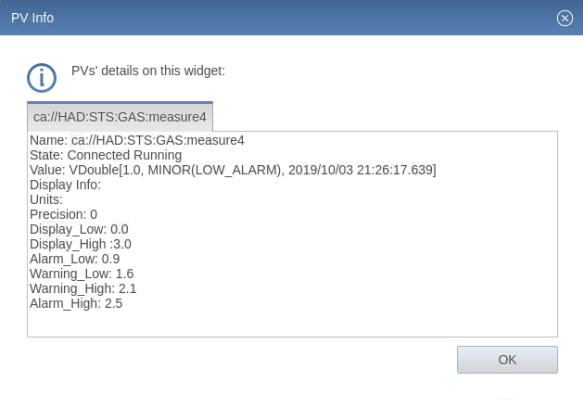
\includegraphics[width=1\textwidth]{images/Minoralarm.PNG}
    \caption{Caption}
    \label{fig:my_label}
\end{figure}
\begin{figure}
    \centering
    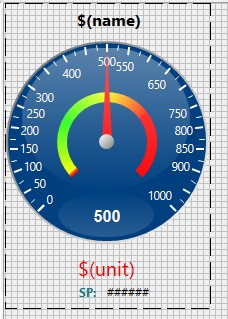
\includegraphics[width=0.4\textwidth]{images/linkcontainer.jpg}
    \caption{Caption}
    \label{fig:my_label}
\end{figure}
\begin{figure}
    \centering
    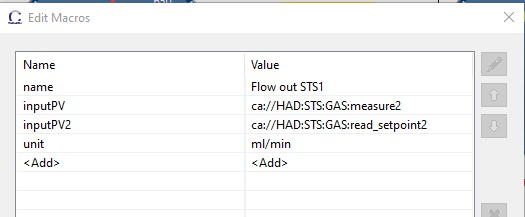
\includegraphics[width=1.0\textwidth]{images/linkcontainer2.jpg}
    \caption{Caption}
    \label{fig:my_label}
\end{figure}
